\PassOptionsToPackage{xetex}{xcolor}
\PassOptionsToPackage{xetex}{graphicx}
\documentclass[a4paper,landscape,headrule,footrule,xetex]{foils}

%%
%%%  Macros
%%%
\newcommand{\logo}{~}
\MyLogo{HG2052 (2020)}
%\newcommand{\Story}{\SHA{HOUN}{The Hound of the Baskervilles}}

\newcommand{\header}[3]{%
\title{\vspace*{-2ex} \Large HG2052
\\\large  Language, Technology and the Internet
\\[2ex] \Large  \emp{#2}}
\author{\blu{Francis Bond}   \\ 
\normalsize  \textbf{Division of Linguistics and Multilingual Studies}\\
\normalsize  \url{http://www3.ntu.edu.sg/home/fcbond/}\\
\normalsize  \texttt{bond@ieee.org}}
\MyLogo{HG2052 (2020)}
\date{#1}
\renewcommand{\logo}{#2}
 \hypersetup{
   pdfinfo={
     Author={Francis Bond},
     Title={#1: #2},
     Subject={HG2052: Language, Technology and the Internet},
     Keywords={Language, Technology, Internet},
     License={CC BY 4.0}
   }
 %  pdfcopyright={Copyright © Francis Bond. Creative Commons 4.0 Attribution License.}
 %  pdflicenseurl={http://creativecommons.org/licenses/by/4.0/}
 }
}


%%
%% Multilingual Stuff
%%
\usepackage[a4paper,landscape,margin=25mm]{geometry}

\usepackage{fontenc}
\usepackage{polyglossia}
\setmainlanguage{english}
\setmainfont{TeX Gyre Pagella}
%\setmainfont{Linux Libertine}
%\setmainfont{Charis SIL}
\newfontfamily{\ipafont}{Gentium}
\newcommand{\ipa}[1]{{\ipafont\selectfont #1}}
\usepackage{xeCJK}

\setCJKmainfont{Noto Sans CJK SC}
\setCJKsansfont{Noto Sans CJK SC}
%\setCJKttfont{Noto Sans CJK SC}
%\setCJKmainfont{WenQuanYi Micro Hei}
%\clearpage
%\setCJKmainfont{AR PL SungtiL GB}

\usepackage[xetex]{xcolor}
\usepackage[xetex]{graphicx}
\newcommand{\blu}[1]{\textcolor{blue}{#1}}
\newcommand{\grn}[1]{\textcolor{green}{#1}}
\newcommand{\hide}[1]{\textcolor{white}{#1}}
\newcommand{\emp}[1]{\textcolor{red}{#1}}
\newcommand{\txx}[1]{\textbf{\textcolor{blue}{#1}}}
\newcommand{\lex}[1]{\textbf{\mtcitestyle{#1}}}

\usepackage{pifont}
\renewcommand{\labelitemi}{\textcolor{violet}{\ding{227}}}
\renewcommand{\labelitemii}{\textcolor{purple}{\ding{226}}}

\newcommand{\subhead}[1]{\noindent\textbf{#1}\\[5mm]}

\newcommand{\Bad}{\emp{\raisebox{0.15ex}{\ensuremath{\mathbf{\otimes}}}}}
\newcommand{\bad}{*}

\newcommand{\com}[1]{\hfill \textnormal{(\emp{#1})}}%
\newcommand{\cxm}[1]{\hfill \textnormal{(\txx{#1})}}%
\newcommand{\cmm}[1]{\hfill \textnormal{(#1)}}%
\usepackage{amssymb}
\usepackage{relsize,xspace}
\newcommand{\into}{\ensuremath{\rightarrow}\xspace}
\newcommand{\ent}{\ensuremath{\Rightarrow}\xspace}
\newcommand{\nent}{\ensuremath{\not\Rightarrow}\xspace}
\newcommand{\tot}{\ensuremath{\leftrightarrow}\xspace}
\usepackage{url}
\usepackage[hidelinks]{hyperref}
\hypersetup{
     colorlinks,
     linkcolor={blue!50!black},
     citecolor={red!50!black},
     urlcolor={blue!80!black}
}
%\usepackage{hyperxmp}
\usepackage{url}
\newcommand{\lurl}[1]{\MyLogo{\url{#1}}}

\usepackage{mygb4e}
\let\eachwordone=\itshape
\newcommand{\lx}[1]{\textbf{\textit{#1}}}
\newcommand{\ix}{\ex\it}

\newcommand{\cen}[2]{\multicolumn{#1}{c}{#2}}
%\usepackage{times}
%\usepackage{nttfoilhead}
\newcommand{\myslide}[1]{%
\foilhead[-25mm]{\raisebox{12mm}[0mm]{\emp{#1}}}%
\leftheader{}%
\MyLogo{\logo}}

\newcommand{\mytask}[1]{%
\foilhead[-25mm]{\raisebox{12mm}[0mm]{\emp{#1}}}
\leftheader{🔍 Hi}%
\MyLogo{\logo}}

\newcommand{\myslider}[1]{\rotatefoilhead[-25mm]{\raisebox{12mm}[0mm]{\emp{#1}}}}
%\newcommand{\myslider}[1]{\rotatefoilhead{\raisebox{-8mm}{\emp{#1}}}}

\newcommand{\section}[1]{\myslide{}{\begin{center}\Huge \emp{#1}\end{center}}}

\usepackage{tcolorbox}
% \newcommand{\task}{\marginpar{\raisebox{-1ex}{\large
%       \tcbox[colframe=red,colback=white,arc=3pt]{\textbf{?}}}}}
% \newcommand{\task}{\marginpar{\raisebox{-1ex}{
%       \hspace{-0.5em}\tcbox[colframe=red,colback=white,arc=3pt]{%
%         \includegraphics[width=1.5em]{pics/detective}}}}}
\newcommand{\task}{\marginpar{\raisebox{-2ex}{
      \hspace{-0.5em}\reflectbox{\includegraphics[width=2em]{pics/detective}}}}}

\usepackage[lyons,j,e,k]{mtg2e}
\renewcommand{\mtcitestyle}[1]{\textcolor{teal}{\textsl{#1}}}
%\renewcommand{\mtcitestyle}[1]{\textsl{#1}}
\newcommand{\chn}{\mtciteform}
\newcommand{\cmn}{\mtciteform}
\newcommand{\iz}[1]{\textup{\texttt{\textcolor{blue}{\textbf{#1}}}}}
\newcommand{\con}[1]{\textsc{#1}}
\newcommand{\gm}{\textsc}
\newcommand{\cmp}[1]{{[\textsc{#1}]}}
\newcommand{\sr}[1]{\ensuremath{\langle}#1\ensuremath{\rangle}}
\usepackage[normalem]{ulem}
\newcommand{\ul}{\uline}
\newcommand{\uul}{\uuline}
\newcommand{\wl}{\uwave}
\newcommand{\vs}{\ensuremath{\Leftrightarrow}~}
%%%
%%% Bibliography
%%%
\usepackage{natbib}
%\usepackage{url}
\usepackage{bibentry}


%%% From Tim
\newcommand{\WMngram}[1][]{$n$-gram#1\xspace}
\newcommand{\infers}{$\rightarrow$\xspace}



\usepackage{rtrees,qtree}
\renewcommand{\lf}[1]{\br{#1}{}}
\usepackage{avm}
%\avmoptions{topleft,center}
\newcommand{\ft}[1]{\textsc{#1}}
\newcommand{\val}[1]{\textit{#1}}
\newcommand{\typ}[1]{\textit{#1}}
\avmfont{\sc}
%\avmvalfont{\sc}
\renewcommand{\avmtreefont}{\sc}
\avmsortfont{\it}


%%% From CSLI book
\newcommand{\mc}{\multicolumn}
\newcommand{\HD}{\textbf{H}\xspace}
\newcommand{\el}{\< \>}
\makeatother
\long\def\smalltree#1{\leavevmode{\def\\{\cr\noalign{\vskip12pt}}%
\def\mc##1##2{\multispan{##1}{\hfil##2\hfil}}%
\tabskip=1em%
\hbox{\vtop{\halign{&\hfil##\hfil\cr
#1\crcr}}}}}
\makeatletter

\newcommand{\sh}[1]{\href{https://www.arthur-conan-doyle.com/index.php?title=#1}{#1}}
\newcommand{\SHA}[2]{\href{https://www.arthur-conan-doyle.com/index.php?title=#1}{\textit{#2}}}


\header{Lecture 5}{Collaboration and Wikis}

\begin{document}
%\begin{CJK}{UTF8}{min}
\bibliographystyle{apalike}
\nobibliography{abb,mtg,nlp,ling}

\maketitle


\myslide{Revision of Email; Usenet; Chat and Blog}

\begin{itemize}
\item All share some characteristics of speech and text
\item Usage norms not fixed
\item Communication methods may disappear before the norms are fixed
\\ (Usenet)
\item Large scale discourse studies still to be done
\item Some genuinely new things
  \begin{itemize}
  \item time-lagged, multi-person conversation
  \item un-edited text
  \end{itemize}
\end{itemize}

\myslide{Email}


\begin{tabular}{ll}
  \textbf{Speech like} & \textbf{Text like} \\ \hline
  \blu{time bound}* &  \blu{space bound} (deletable) \\
  \blu{spontaneous}* & \blu{contrived}* \\
  face-to-face & \blu{visually decontextualized} \\
  \blu{loosely structured}* & \blu{elaborately structured}* \\
  \blu{socially interactive}* & \blu{factually communicative} \\  
  immediately revisable & \blu{repeatedly revisable}* \\
  prosodically rich & graphically rich * \\
\end{tabular}


\myslide{Usenet (asynchronous)}


\begin{tabular}{ll}
  \textbf{Speech like} & \textbf{Text like} \\ \hline
  \blu{time bound}* &  \blu{space bound} \\
  \blu{spontaneous}* & \blu{contrived}* \\
  face-to-face & \blu{visually decontextualized} \\
  \blu{loosely structured}* & elaborately structured \\
  \blu{socially interactive}* & \blu{factually communicative} \\  
  immediately revisable & repeatedly revisable \\
  prosodically rich & graphically rich  \\
\end{tabular}



\myslide{Chat (synchronous)}


\begin{tabular}{ll}
  \textbf{Speech like} & \textbf{Text like} \\ \hline
  \blu{time bound}* &  \blu{space bound} \\
  \blu{spontaneous}* & contrived \\
  face-to-face & \blu{visually decontextualized} \\
  \blu{loosely structured}* & elaborately structured \\
  \blu{socially interactive}* & \blu{factually communicative} \\  
  immediately revisable & repeatedly revisable \\
  prosodically rich & graphically rich  \\
\end{tabular}


\myslide{Blogs}


\begin{tabular}{ll}
  \textbf{Speech like} & \textbf{Text like} \\ \hline
  time bound &  \blu{space bound} \\
  \blu{spontaneous}* & \blu{contrived}* \\
  face-to-face & \blu{visually decontextualized} \\
  \blu{loosely structured}* & \blu{elaborately structured}* \\
  \blu{socially interactive}$^{comments}$ & \blu{factually communicative} \\  
  immediately revisable & \blu{repeatedly revisable}* \\
  prosodically rich & graphically rich * \\
\end{tabular}


\section{Collaboration and Wikis}

\myslide{Overview}
\MyLogo{}
\begin{itemize}
\item Version Control Systems
\item Wikipedia
\item Some issues within Wikipedia
\item Licensing and Ownership 
\end{itemize}

\myslide{Versions, Revisions, Authorship}

\begin{itemize}
\item Many works have multiple versions
\item Before writing, every production was different
\item With writing, every copy was different (before printing)
\item The same source may have multiple translations
\item Authors (and Editors and Publishers) revise text
  \begin{itemize}
  \item Examples?
  \end{itemize}
\item Computers can store multiple versions together
\end{itemize}


\myslide{Revision Control Systems}

\begin{itemize}
\item Versioning file systems
  \begin{itemize}
  \item  every time a file is opened, a new copy is stored
  \end{itemize}
\item CVS (Concurrent Versioning System), Subversion, Git
  \begin{itemize}
  \item changes to a collection of files are tracked
  \item simultaneous changes are merged
  \item github is a popular interface:
    \href{https://github.com/fcbond}{github.com/fcbond},
    \href{https://github.com/bond-lab}{github.com/bond-lab} 
  \end{itemize} 
\item Revision Tracking
  \begin{itemize} 
  \item Revisions are stored within a file (MS Word, Google Docs)
  \end{itemize}
\item Authorship in shared writing (who wrote what?)
\end{itemize}

\myslide{svn blame}
\MyLogo{Aliases: praise, annotate, ann}
\begin{tiny}
\begin{verbatim}
    92     siegel 
     2     siegel ;;;;;;;;;;;;;;;;;;;;;;;;;;;;;;;;;;;;;;;;;;;;;;;;;;;;;;;;;;;;;;;;;;;;;;;;;;;;;;;
     2     siegel ;;;        file: japgram
     2     siegel ;;;  written by: Melanie Siegel/Emily Bender
     2     siegel ;;;;;;;;;;;;;;;;;;;;;;;;;;;;;;;;;;;;;;;;;;;;;;;;;;;;;;;;;;;;;;;;;;;;;;;;;;;;;;;
     2     siegel ;;; author            | date        | modification
     2     siegel ;;; ------------------|-------------|------------------------------------------
    94       bond ;;;Melanie Siegel (MS)|             | Emily Bender (ERB), Francis Bond (FCB), 
    94       bond ;;;                   |             | Chikara Hashimoto (CH),  
   421 michael.goodman ;;;                   |             | Takaaki Tanaka (TT), Akira Ohtani (AO),
   421 michael.goodman ;;;                   |             | Michael Goodman(MWG)
     2     siegel ;;;;;;;;;;;;;;;;;;;;;;;;;;;;;;;;;;;;;;;;;;;;;;;;;;;;;;;;;;;;;;;;;;;;;;;;;;;;;;;
     2     siegel 
     2     siegel ;Rules for sentence chains or single sentences
     2     siegel 
     2     siegel ;declarative sentence, finite verb
     2     siegel 
   334 francis_bond ; <ex>(do-parse-tty "食べる")</ex>
   334 francis_bond utterance_rule-decl-finite := utterance-sf-type &
   424 francis_bond  [SYNSEM.LOCAL.CAT.HEAD.SMOD decl, 
   334 francis_bond   C-CONT.HOOK.INDEX.SF prop,
   334 francis_bond   ARGS.FIRST.SYNSEM [LOCAL.CAT.HEAD [MODUS uttmodus, 
   334 francis_bond 				     FIN +],
   334 francis_bond 		     NON-LOCAL.QUE <! !>]]. 

\end{verbatim}
\end{tiny}

It shows the revision, who committed it and which lines were affected.


\myslide{Tracking Changes in MS Word}
\MyLogo{}
\begin{center}
  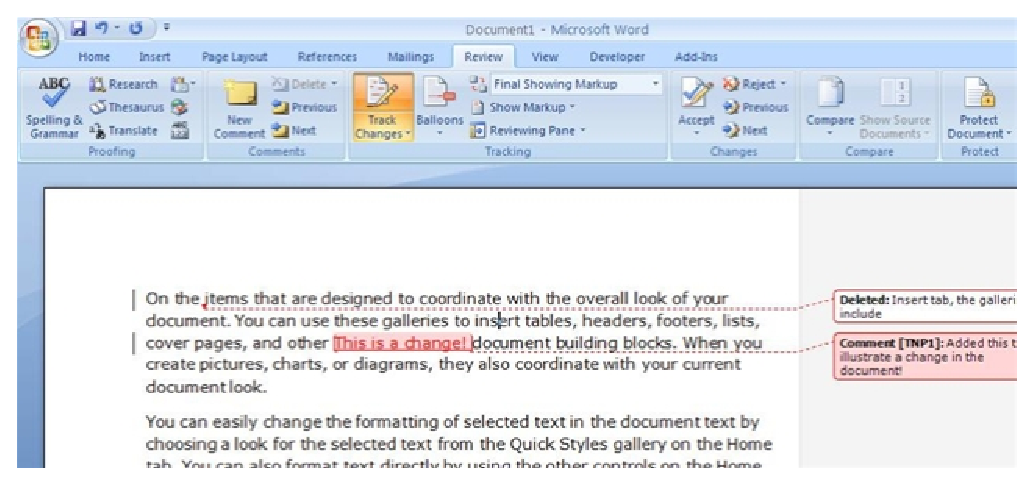
\includegraphics[width=\textwidth]{../pics/word-track-changes}
\end{center}

\myslide{Collaborative Authoring Strategies}

\begin{itemize}
\item Everyone writes a version and someone merges
\item Pass a file round
\item Have a copy at a shared repository (checkout/commit)
\item Allow simultaneous (nearly) editing online
  \\ only made possible by fast reliable internet
  \begin{itemize}
  \item  \blu{the wiki}: a website that allows the easy creation and editing of any number of interlinked web pages via a web browser using a simplified markup language or a WYSIWYG text editor
  \item Ward Cunningham, the developer of the first wiki software, WikiWikiWeb, originally described it as "the simplest online database that could possibly work."
  \item ``Wiki'' is a Hawaiian word for "fast"
  \end{itemize}
\end{itemize}


\myslide{Does collaborative authoring change language?}

\begin{itemize}
\item No one has measured this (as far as I know)
  \begin{itemize}
  \item Are sentences longer/shorter?
  \item Is the writing easier/harder to follow?
  \item Is it more/less pleasant to read?
  \item Does it have more/fewer errors?
  \end{itemize}
  Good topic for an undergraduate thesis, \ldots
\item Collaboration is sometimes in large chunks, sometimes in small
  chunks, sometimes at the level of formatting
\item This is an untapped area of study
\item For computer science, the ability to make changes, share and
  revert easily has made a big difference to how work is done --- I
  think this will also change at least some authorship (my research
  papers are written like this)
\end{itemize}

\section{Wikis and Wikipedia}

\myslide{The original wiki}
\begin{center}
  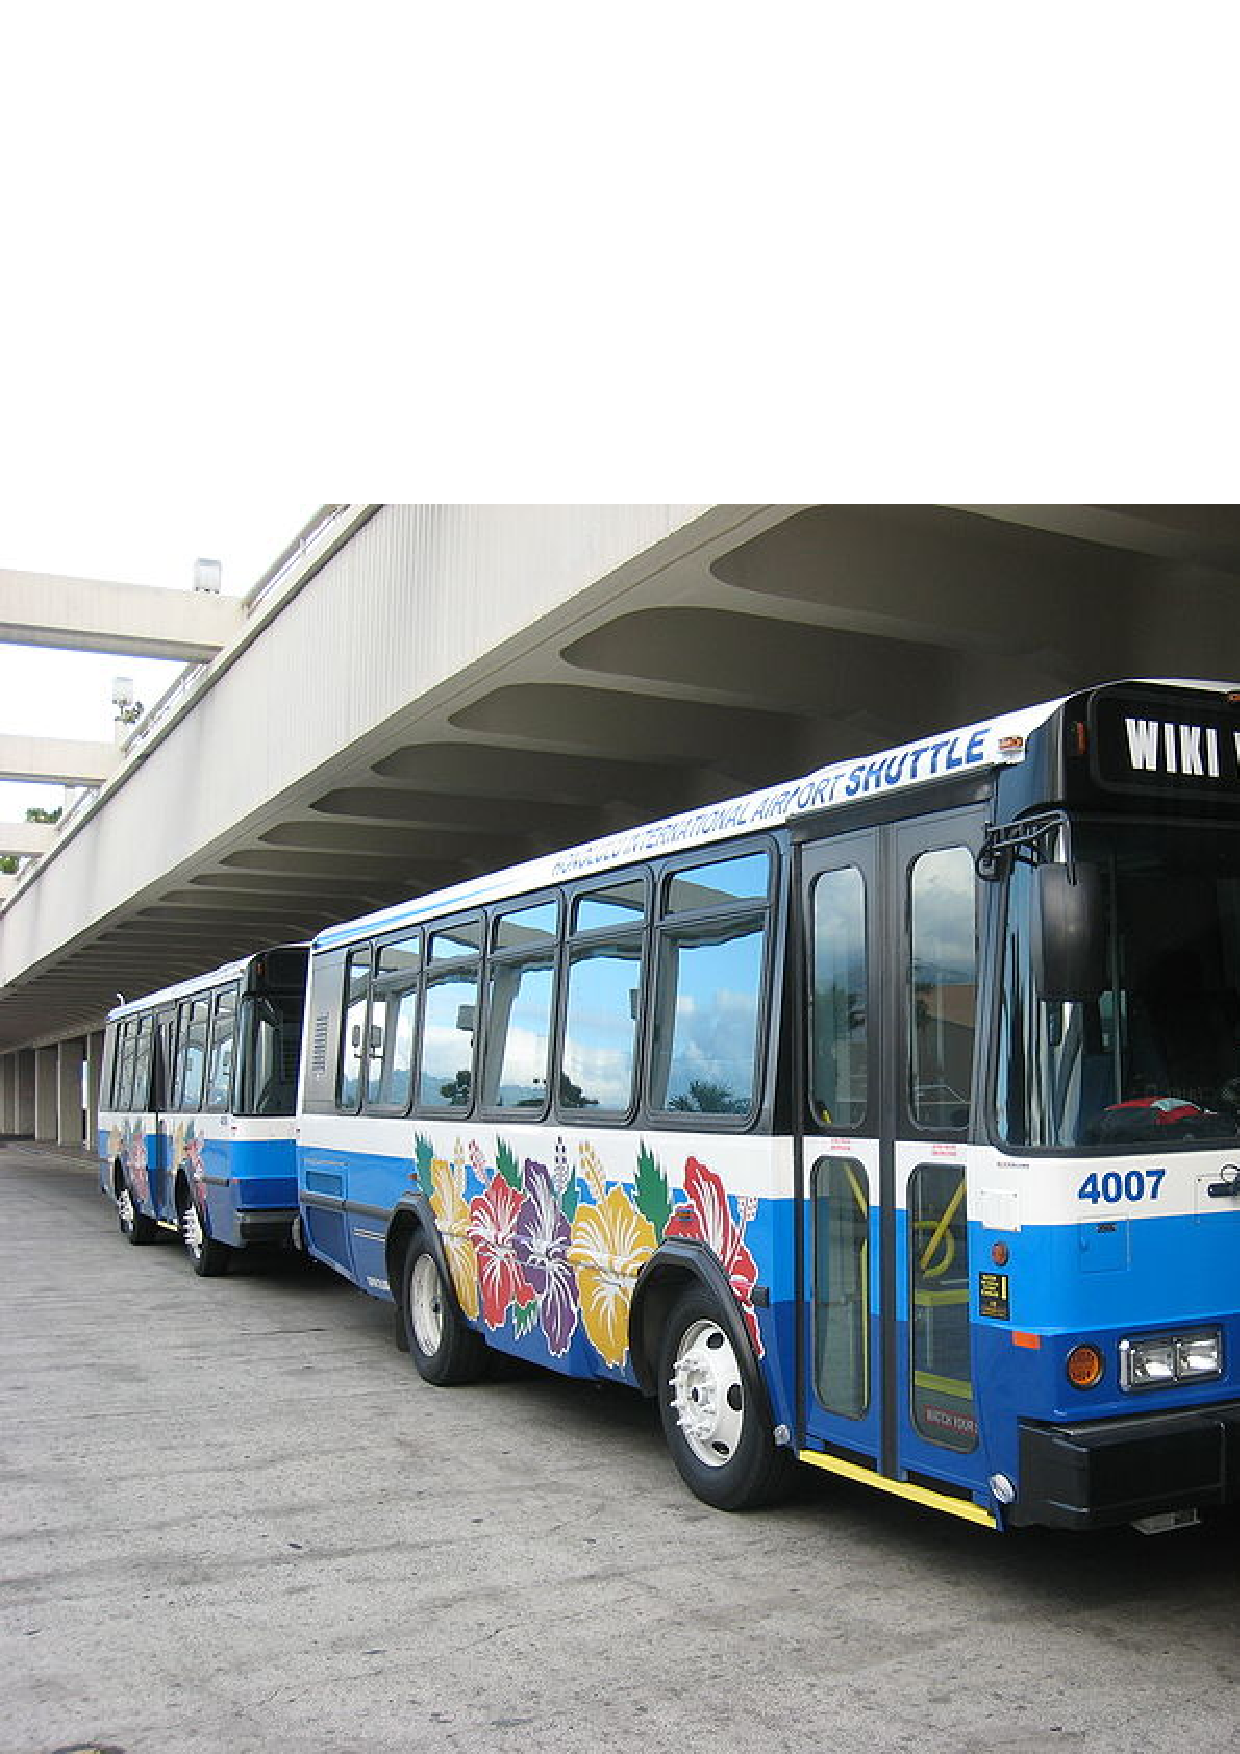
\includegraphics[height=\textheight]{../pics/wiki-shuttle}
\end{center}


\myslide{Wikipedia}
\begin{itemize}
\item Nupedia
\item Lowering the barrier to entry
\item Who edits what?
\item Who edits what when?
\item How to ensure quality?
\item Research with Wikipedia
\end{itemize}


\myslide{Nupedia}

\begin{itemize}
\item Build a free encyclopedia written by experts
\\ true experts in their fields who with few exceptions possess PhDs
\item Nupedia had a seven-step editorial process, consisting of:
  \begin{enumerate}
  \item  Assignment
  \item  Finding a lead reviewer
  \item  Lead review
  \item  Open review
  \item  Lead copyediting
  \item  Open copyediting
  \item  Final approval and markup
  \end{enumerate}
\item Wikipedia was a side-project to allow collaboration on articles prior to entering the peer review process (3.5)
 \item Nupedia never got beyond 24 articles
 \end{itemize}
 
\myslide{Lowering the barrier to entry}

\begin{itemize}
\item Wikipedia makes it easy to share your knowledge
  \begin{itemize}
    \item People like to do this
  \end{itemize}
\item You don't even have to register
\item Getting content is hard --- so it is crucial that it is easy to add information
\end{itemize}


\myslide{Wikipedia has been an enormous success}

\begin{itemize}%\addtolength{\itemsep}{-1ex}
\item
  \href{https://www.theguardian.com/commentisfree/2018/sep/02/in-hysterical-world-wikipedia-ray-of-light-truth}{In
    a hysterical world, Wikipedia is a ray of light – and that's the
    truth}: It has been the butt of jokes for years, but the online
  encyclopedia represents mankind at its very best (John Naughton, The
  Guardian 2020)
\item
  \href{https://www.theguardian.com/technology/2020/sep/18/wikipedia-edits-have-massive-impact-on-tourism-say-economists}{Wikipedia
    edits have massive impact on tourism, say economists}: Adding a
  few paragraphs and photos can boost revenue by £100,000 for small
  cities (The Guardian, 2020)
\item Wikipedia is open content, released under a free license. Knowing this encourages people to contribute; they know it's a public project everyone can use.
\item Wikipedia's neutral point of view policy makes it an excellent place to gain a quick understanding of controversial topics. 
\item Articles steadily become more polished as they develop, \ldots
 
\end{itemize}

Quoted directly from \href{https://en.wikipedia.org/wiki/Wikipedia:Why_Wikipedia_is_so_great}{Wikipedia:Why Wikipedia is so great} unless otherwise noted.

\myslide{Who writes Wikipedia: the in-crowd}

\begin{itemize}
\item 50\% of all the edits are done by just .7\% of the users (524 people)
\item 73\% of all the edits are done by 2\%  (1,400 people)
  \begin{flushright}
    Jimmy Wales (Talk at Stanford, 2005)
  \end{flushright}
\end{itemize}

\emp{Most edits are done by insiders!}
%%% Fixme add NYT article

\begin{itemize}
\item
  \href{https://en.wikipedia.org/wiki/Wikipedia:Who_writes_Wikipedia?}{Who
  Writes Wikipedia?}
\item 
\href{https://www.washingtonpost.com/lifestyle/magazine/meet-the-most-prolific-contributor-to-the-english-version-of-wikipedia/2018/10/02/a6497a74-9411-11e8-a679-b09212fb69c2_story.html?utm_term=.18bfc6ecda09}{Meet
  the most prolific contributor to the English version of wikipedia}
Washington Post (2019)
\end{itemize}


\myslide{Who writes Wikipedia: the out-crowd}

A close look at one page (\textbf{Alan Alda}):

If you just count edits (7 of the top 10) are registered users who
(all but 2) have made thousands of edits to the site. Indeed, \#4 has
made over 7,000 edits while \#7 has over 25,000.

When you count letters: few of the contributors (2 out of the top 10)
are even registered and most (6 out of the top 10) have made less than
25 edits to the entire site. In fact, \#9 has made exactly one edit —
this one!

A great many people add a bit of content about something they know
about, and a few people make many small changes to make it conform to
wikipedia style.

\emp{Most content is added by outsiders!}


Aaron Swartz (2006) \href{http://www.aaronsw.com/weblog/whowriteswikipedia}{Who Writes Wikipedia?} 
\textit{RAW THOUGHT} (weblog, accessed 2023-10-09)


Denise Anthony, Sean W Smith and Tim Williamson (2007) "\href{https://digitalcommons.dartmouth.edu/cs_tr/306}{The Quality of Open Source Production: Zealots and Good Samaritans in the Case of Wikipedia}" (2007). Computer Science Technical Report TR2007-606. 

\myslide{WIERD Male Biases}

\begin{itemize}
\item  \href{https://www.theguardian.com/technology/2018/jul/29/the-five-wikipedia-biases-pro-western-male-dominated}{Wikipedia
    biases: 
Research exposes the male-dominated, pro-western worldview of the online encyclopedia}
  Poppy   Noor 2018-07-27
\item Mainly Western
\item Sources mainly in the language of the wikipedia
\item Liberal bias              %
\item  \href{https://www.washingtonpost.com/lifestyle/style/history-has-a-massive-gender-bias-well-settle-for-fixing-wikipedia/2019/02/15/b2537640-3163-11e9-86ab-5d02109aeb01_story.html?utm_term=.7d4409494928}{History
    has a massive gender bias. We'll settle for fixing Wikipedia}
  Monica Hesse 2019-02-17
\item Only about 18 percent of Wikipedia's biographical articles are
  about women.
\item  That's up 3 percent from a few years ago,
\item ``contributors are majority Western and mostly male, and these
  gatekeepers apply their own judgment and prejudices'' (Wikipedia Foundation)
\end{itemize}

\myslide{The five pillars of Wikipedia}
\MyLogo{\url{Wikipedia:Five pillars}}
\begin{enumerate}
\item Wikipedia is an online encyclopedia
\item Wikipedia has a neutral point of view.
\item Wikipedia is free content
\item Wikipedians should interact in a respectful and civil manner
\item Wikipedia does not have firm rules
\end{enumerate}
\begin{quote}
  the core aim of the Wikimedia Foundation, is to get a free
  encyclopedia to every single person on the planet.
\begin{flushright}
  Jimmy Wales TED talk 2006
\end{flushright}
\end{quote}






\myslide{Encyclopedia}

\begin{large}
  Wikipedia combines many features of general and specialized encyclopedias, almanacs, and gazetteers. Wikipedia is not a soapbox, an advertising platform, a vanity press, an experiment in anarchy or democracy, an indiscriminate collection of information, or a web directory. It is not a dictionary, a newspaper, or a collection of source documents, although some of its fellow Wikimedia projects are.
\end{large}
\myslide{NPOV} 

\begin{large}
We strive for articles in an impartial tone that document and explain
major points of view, giving due weight for their prominence. We avoid
advocacy, and we characterize information and issues rather than
debate them. In some areas there may be just one well-recognized point
of view; in others, we describe multiple points of view, presenting
each accurately and in context rather than as ``the truth'' or ``the best
view''. All articles must strive for verifiable accuracy, citing
reliable, authoritative sources, especially when the topic is
controversial or is about a living person. Editors' personal
experiences, interpretations, or opinions do not belong on Wikipedia.
\end{large}

\myslide{Free} 

\begin{large}
  Since all editors freely license their work to the public, no editor owns an article and any contributions can and may be mercilessly edited and redistributed. Respect copyright laws, and never plagiarize from any sources. Borrowing non-free media is sometimes allowed as fair use, but strive to find free alternatives first.
\end{large}

\begin{itemize}
\item licensed under the \textit{Creative Commons Attribution-ShareAlike License}
\end{itemize}


\myslide{Code of conduct and etiquette} 

\begin{large}
  Respect your fellow Wikipedians, even when you disagree. Apply Wikipedia etiquette, and do not engage in personal attacks. Seek consensus, avoid edit wars, and never disrupt Wikipedia to illustrate a point. Act in good faith, and assume good faith on the part of others. Be open and welcoming to newcomers. Should conflicts arise, discuss them calmly on the appropriate talk pages, follow dispute resolution procedures, and consider that there are over 6,726,000 other articles on the English Wikipedia to improve and discuss.
\end{large}

\myslide{Ignore all rules (IAR)} 

\begin{large}
  Wikipedia has policies and guidelines, but they are not carved in stone; their content and interpretation can evolve over time. The principles and spirit matter more than literal wording, and sometimes improving Wikipedia requires making exceptions. Be bold, but not reckless, in updating articles. And do not agonize over making mistakes: (almost) every past version of a page is saved, so mistakes can be easily corrected.
\end{large}


\myslide{Quality Control}
\MyLogo{}
\begin{itemize}
\item How is quality maintained?
\item Some people regularly check the \blu{new changes} page
\item Many people watch pages of interest to them
\item All information is stored and accessible
\item Wikiscanner (an outside project links editors to the real world)
  \begin{itemize}
  \item On November 17th, 2005, an anonymous Wikipedia user deleted 15 critical 
    paragraphs from an article on e-voting machine-vendor Diebold
  \item The editor was anonymous but the changes came from an IP
    address reserved for the corporate offices of Diebold
  \end{itemize}
\end{itemize}
% \item 

% You can see which IP address are linked to which organization and then
% see where they have edited wikipedia!  The openness of the data (wiki
% records who edited what) guards against 

%  Japanese officials chided for
% editing Wikipedia Probe found six bureaucrats spent work hours editing
% unrelated topics

% \url{http://www.msnbc.msn.com/id/21151261/}

\myslide{Wikipedia vs Britannica}
\MyLogo{\url{http://www.nature.com/nature/journal/v438/n7070/full/438900a.html}}

\begin{itemize}
\item \textit{Nature} study compared 42 articles reviewed by three experts

\item The average scientific entry in Wikipedia contained four errors
  or omissions, while Britannica had three.
\item Of eight ``serious errors'' the reviewers found — including misinterpretations of important concepts — four came from each source
\item Wikipedia is good on pop culture and contemporary technology
  because Wikipedia's stable of dedicated volunteers tend to have more
  collective expertise in such areas.
\item Wikipedia  tends to lag when it comes to topics touching on the humanities 
  \begin{itemize}
  \item Techies are on-line more, and share information more readily.
  \end{itemize}
\end{itemize}

\myslide{Problems with Wikipedia}
\MyLogo{From \url{http://simple.wikipedia.org/wiki/Problems_of_Wikipedia}}
\begin{itemize}
\item Anyone can change an article in Wikipedia. Some articles in
  Wikipedia may not be entirely true and accurate, instead displaying
  a hoax or a false information.
\item In particular, there is a problem of vandalism. Some  is obvious,
  other forms  may be difficult to see.
\item People who have a strong opinion about a subject will try to
  control the articles about that subject.
\item Not all facts are backed by sources, not all sources are
  reliable, and not all are checked.
\item Not all editors are competent or pleasant. 
\end{itemize}

\myslide{Problems with Wikipedia (II)}
\MyLogo{\url{http://xkcd.com/214/} The Problem with Wikipedia}
\begin{center}
  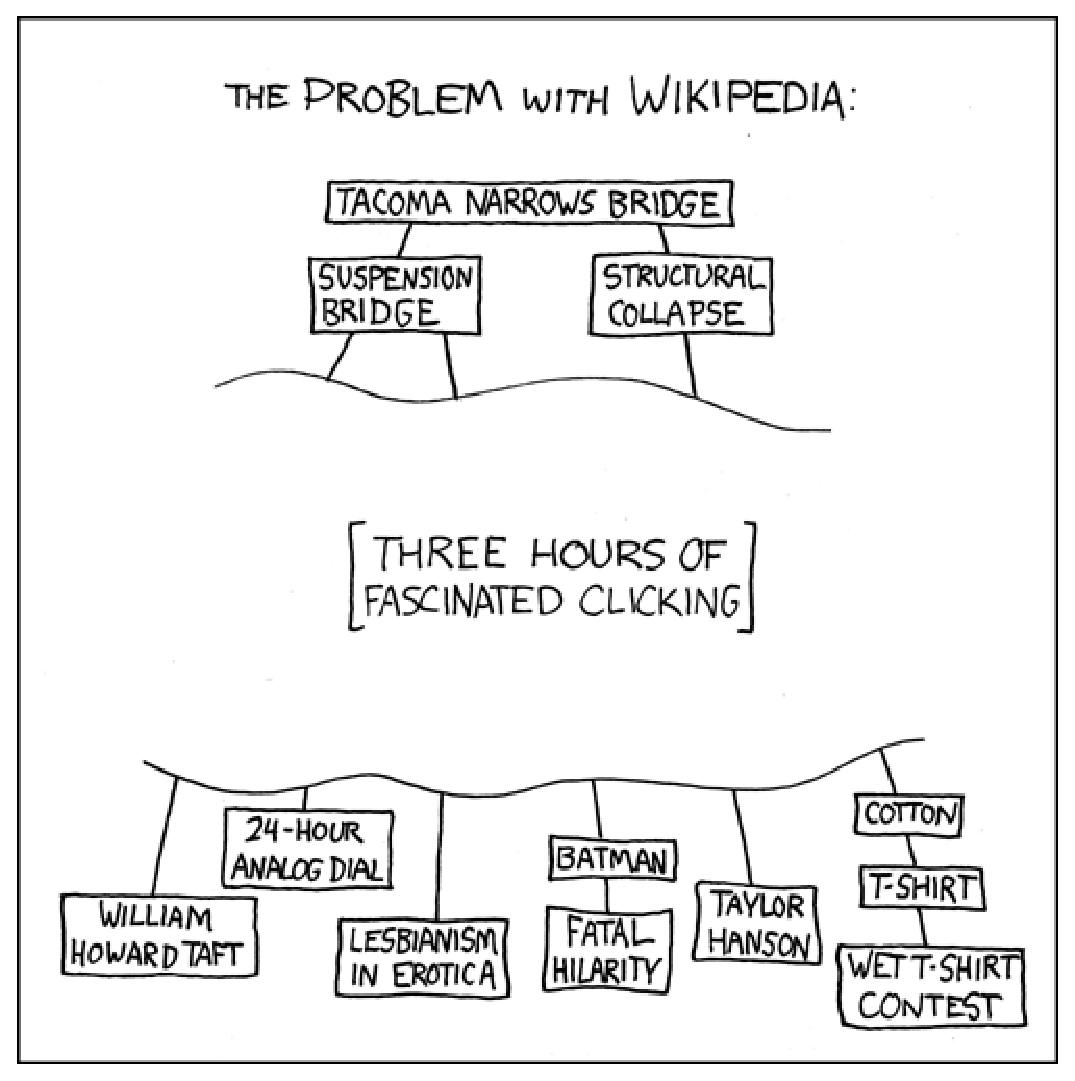
\includegraphics[height=\textheight]{../pics/xkcd-problem_wiki}
\end{center}

\myslide{Problems with Wikipedia (III)}
\MyLogo{\url{http://www.technologyreview.com/featuredstory/520446/the-decline-of-wikipedia/}}

\begin{large}
  The motto of Wikipedia should be 
  \begin{quote}
    ``the encyclopedia that anyone who understands the norms,
    socializes him or herself, dodges the impersonal wall of
    semi-automated rejection and still wants to voluntarily contribute
    his or her time and energy can edit.''
  \end{quote}
\end{large}

\myslide{Research with Wikipedia}
\MyLogo{}

\begin{itemize}
\item Extraction
  \begin{itemize}
  \item Mining Wikipedia for structured knowledge
  \end{itemize}
\item Translation
  \begin{itemize}
  \item Mining cross-wiki links for translations 
  \end{itemize}
\item \href{http://moin.delph-in.net/WeScience}{WeScience}
  \begin{itemize}
  \item Using Wikipedia as a vast corpus
  \end{itemize}
\item Training Data for Large Language Models
\end{itemize}

\myslide{Other Wikis}
%%% FIXME link
\begin{itemize}
\item DELPH-IN wiki (Deep Linguistic Processing for HPSG Initiative)
\item Wiktionary
\item the Wiki of the Association for Computational Linguistics
\item Conservapedia
\item[\ldots]
\end{itemize}


\myslide{What is a good article?}
\MyLogo{\url{Wikipedia:Good_article_criteria}}

\begin{enumerate}
\item Well-written
\item Factually accurate and verifiable
\item Broad in its coverage
\item Neutral
\item Stable
\item Illustrated, if possible, by images
\end{enumerate}

\myslide{Well-written}

\begin{itemize}
\item  the prose is clear and concise, and the spelling and grammar are correct
  \begin{itemize}
  \item Some students have been a bit sloppy about this in the past
  \end{itemize}
\item  it complies with the manual of style guidelines for 
  \begin{itemize}
  \item lede/lead sections
  \item layout
  \item words to watch
  \item fiction
  \item list incorporation
  \end{itemize}
\end{itemize}

\myslide{Factually accurate and verifiable}

\begin{itemize}
\item  it provides references to all sources of information in the section(s) dedicated to the attribution of these sources according to the guide to layout;
\item  it provides in-line citations from reliable sources for direct quotations, statistics, published opinion, counter-intuitive or controversial statements that are challenged or likely to be challenged, and contentious material relating to living persons
--- science-based articles should follow the scientific citation guidelines;
\item it contains no original research.
  \begin{itemize}
  \item different from a research paper
  \end{itemize}
\end{itemize}

\myslide{Broad in its coverage}
\begin{itemize}
\item  it addresses the main aspects of the topic
\item  it stays focused on the topic without going into unnecessary detail
\end{itemize}

\myslide{Neutral, Stable and Illustrated}
\begin{itemize}
\item  it represents viewpoints fairly and without bias
\item it does not change significantly from day to day because of an ongoing edit war or content dispute
\item  images are tagged with their copyright status, and valid fair use rationales are provided for non-free content
\item  images are relevant to the topic, and have suitable captions.
\end{itemize}




\myslide{Edit Wars}
\MyLogo{}
An edit war occurs when editors who disagree about some aspect of the
content of a page repeatedly override each other's contributions,
rather than try to resolve the disagreement by discussion.

Edit warring is unconstructive and creates animosity between editors,
making it harder to reach a consensus as to the right way to improve
the encyclopedia. Users who engage in edit wars risk being blocked or
even banned from editing.

\emp{The three-revert rule} (3RR): do not perform more than three reverts on a
single page within a 24-hour period. Breaking this rule is
sufficient—but not necessary—to warrant a block for edit warring.

\myslide{Lamest Edit Wars}
\MyLogo{\url{https://en.wikipedia.org/wiki/Wikipedia:Lamest_edit_wars}}



\begin{description}
\item [German Wikipedia's Article on Danube Tower]
Is the Danube Tower "an observation tower" or "a television and observation tower"? This edit war was so lame that it got covered in Der Spiegel.
\item [Template:WikiProject Computer science]
58kb of talk page debate plus a user block over how to copyedit a two line statement.
\item [Sea of Japan]
Should it be called the Sea of Japan, the East Sea, or even the East Sea of Korea? Are both names valid, and if so, should the article be named Sea of Japan (East Sea) or Sea of Japan / East Sea? Or is the actual most common English and international name Sea of Japan (East Sea), parentheses and all? Should the dispute page be called the Sea of Japan naming dispute, or the Naming dispute over the body of water between Japan and Korea and the Russian Far East? \ldots
\end{description}

\section{Access and Ownership}
\MyLogo{}

\myslide{Licenses and Ownership}

\begin{itemize}
\item Copyright
\item Copyleft
\item Creative Commons
\item Ownership of a Language
\end{itemize}

\myslide{Copyright}

\begin{itemize}
\item State assigned monopoly to encourage an author so that the author of a
  work may reap the fruits of his or her intellectual creativity for a
  limited period of time.
\item Copyright is a form of protection provided by the laws of a
  country for original works of authorship, including literary,
  dramatic, musical, architectural, cartographic, choreographic,
  pantomimic, pictorial, graphic, sculptural, and audiovisual
  creations.
\item First legislated in England (1710). There was no automatic copyright protection for unpublished works.
\item Currently 70 years after death of author (varies from country to country)
\item What is the best balance?
\end{itemize}

\myslide{Copyleft}

\begin{itemize}
\item the practice of using copyright law to offer the right to distribute copies and modified versions of a work and requiring that the same rights be preserved in modified versions of the work.
  \begin{itemize}
  \item You can redistribute it if and only if others can also
  \end{itemize}
\item \blu{copyleft} is a general method for making a program (or other work) free, and requiring all modified and extended versions of the program to be free as well
\item Gnu General Public License (GPL)
 \\ (Richard Stallman/Free Software Foundation)
\end{itemize}


\myslide{Creative Commons (CC): some rights reserved}
\MyLogo{\url{https://creativecommons.org/}}
\begin{description}
\item [Attribution (BY)] requiring attribution to the original author
\item [Share Alike (SA)] allowing derivative  works under the same or
  a similar license (later version or different jurisdiction)\com{copyleft}
\item [Non-Commercial (NC)] requiring the work not be used for commercial purposes
\item [No Derivative Works (ND)] allowing only the original work, without derivatives
\end{description}

\begin{itemize}
\item Wikipedia is \textbf{CC BY SA}
\item These slides are \textbf{CC BY}
\end{itemize}

% \myslide{Conclusion}

% \begin{itemize}
% \item The web is changing what humanity can do with language
% \item It is not clear if it is changing what individual humans do
% \end{itemize}

%%% FIXME add NTU stuff
\myslide{Open Science}
\begin{itemize}
\item the movement to make scientific research, data and dissemination accessible to all levels of an inquiring society, amateur or professional
  \begin{itemize}
  \item publishing open research
  \item making data available
  \item making tools (mainly software available)
  \end{itemize}
\item \href{https://openscience.upol.cz/en/}{Palacký University Open Science Page}
\item \href{http://research.ntu.edu.sg/rieo/RI/Pages/Research-Data-Policies.aspx}{NTU's policy}: ``The final research data from projects carried out
  at NTU shall be made available for sharing (via the NTU Data
  Repository) unless there are prior formal agreements with external
  collaborators and parties on non-disclosure or proprietary use of
  the data.''  NTU's default license is CC-BY-NC 
\end{itemize}

\myslide{Who owns a language?}
\MyLogo{the Aboriginal Studies Electronic Data Archive FAQ \url{www1.aiatsis.gov.au/ASEDA/faq.html}}
\begin{itemize}
\item [Q]: Why do depositors restrict access to material?
\item [A]: There are a variety of reasons why a depositor might
  specify an access restriction.  The people they have recorded may
  specify that they want their material kept safe, but not
  distributed.  Occasionally depositors restrict access for a limited
  time until they have checked the material, to see if it is accurate
  enough for distribution or publication \,—\,authors are concerned that inaccurate information may take on a life of its own.  Some information (though only a small fraction of ASEDA holdings) is restricted because it is secret/sacred.
\newpage
\item [Q]: Why do speakers restrict access to material in their languages?
\item [A]: Many speakers of endangered languages consider that their language is their intellectual property, passed down to them from their ancestors.  If it is made freely available to others, then their rights in that language can be diminished.  Usually they do not want strangers to use words and sentences of their languages in an inappropriate way, and want to be consulted prior to public use. 
\end{itemize}


\myslide{Conclusions}
\MyLogo{}
\begin{itemize}
\item Version Control Systems
  \begin{itemize}
  \item Allow asynchronous cooperation, blur ownership
  \end{itemize}
\item Wikipedia
\item Some issues within Wikipedia
\item Licensing and Ownership 
\end{itemize}


\myslide{Project}

\begin{itemize}
\item Now let's edit
\end{itemize}

\end{document}


%%% Local Variables: 
%%% coding: utf-8
%%% mode: latex
%%% TeX-PDF-mode: t
%%% TeX-engine: xetex
%%% End: 
